\documentclass[12pt,a4paper,openright,twoside]{book}
\usepackage[utf8]{inputenc}
\usepackage{phd-thesis}
\usepackage{code-lstlistings}
\usepackage{notes}
\usepackage{shortcuts}

\mainlinespacing{1.241} % line spacing in mainmatter, comment to default (1)

\begin{document}
	
\frontmatter
\input{front}

\begin{abstract}	
Max 2000 characters, strict.
\end{abstract}

\begin{dedication} % this is optional
Optional. Max a few lines.
\end{dedication}

\begin{acknowledgements} % this is optional
Optional. Max 1 page.
\end{acknowledgements}

%----------------------------------------------------------------------------------------
\tableofcontents   
\listoffigures     % (optional) comment if empty
\lstlistoflistings % (optional) comment if empty
%----------------------------------------------------------------------------------------

\mainmatter

%----------------------------------------------------------------------------------------
\chapter{Introduction}
\label{chap:introduction}
%----------------------------------------------------------------------------------------

Write your intro here.
\sidenote{Add sidenotes in this way. They are named after the author of the thesis}

\paragraph{Structure of the Thesis}

\note{Racall to describe the structure of the paper}


\part{Background}

%----------------------------------------------------------------------------------------
\chapter{Context and Motivation}
%----------------------------------------------------------------------------------------
\section{Collective Adaptive Systems}
\section{Self-* Systems}
\section{Edge-Cloud Continuum}


%----------------------------------------------------------------------------------------
\chapter{Macroprogramming}
%----------------------------------------------------------------------------------------
\section{Conceptual Framework}
\section{Field Calculus}
\section{Aggregate Computing}

%----------------------------------------------------------------------------------------
\chapter{Federated Learning}
%----------------------------------------------------------------------------------------
\section{Training Dynamics}
\section{Decentralized Architectures}
\section{Data Heterogeneity}
\section{Clustered Federated Learning}

%----------------------------------------------------------------------------------------
\chapter{Reinforcement Learning}
%----------------------------------------------------------------------------------------
\section{Single Agent}
\section{Multi Agent}
\section{Scalability in RL}
\section{Decentralized RL}

%----------------------------------------------------------------------------------------
\chapter{Other ML Fancy Stuff}
%----------------------------------------------------------------------------------------
\section{Graph Neural Networks}
\section{Random Network Distillation}
\section{Sparsification}
\section{Continual Learning}



\part{Contribution}

%----------------------------------------------------------------------------------------
\chapter{Closing the gap between AC and AI}
%----------------------------------------------------------------------------------------
\section{Motivation}
\section{Phyelds}
\section{Evaluation}
\section{Related Works}

%----------------------------------------------------------------------------------------
\chapter{Federated Learning}
%----------------------------------------------------------------------------------------
\section{Motivation}
\section{Field-Based Coordination for FL}
\subsection{Formalization}
\subsection{Self-* properties}
\subsection{Evaluation}
\section{Sparsification in FL}
\subsection{Formalization}
\subsection{Evaluation}
\section{Clustered Continual Federated Learning under Spatial and Temporal Drift}
\subsection{Formalization}
\subsection{Evaluation}
\section{Related Works}


%----------------------------------------------------------------------------------------
\chapter{Scalable Reinforcement Learning}
%----------------------------------------------------------------------------------------
\section{Motivation}
\section{Neighbor-Based Strategies for Decentralized Reinforcement Learning}
\section{Scaling Multi-Agent Reinforcement Learning with GNNs}
\section{Evaluation}
\section{Related Works}

%----------------------------------------------------------------------------------------
\chapter{Adptive Task-Placement across the Edge-Cloud Continuum}
%----------------------------------------------------------------------------------------
\section{Motivation}
\section{Proposed method: IDHGQL}
\section{Evaluation}
\section{Related Works}

%----------------------------------------------------------------------------------------
\chapter{Wrap Up}
%----------------------------------------------------------------------------------------
\section{Conclusions}
\section{Future Works}

% \chapter{State of the art}

% I suggest referencing stuff as follows: \cref{fig:random-image} or \Cref{fig:random-image}

% \begin{figure}
%     \centering
%     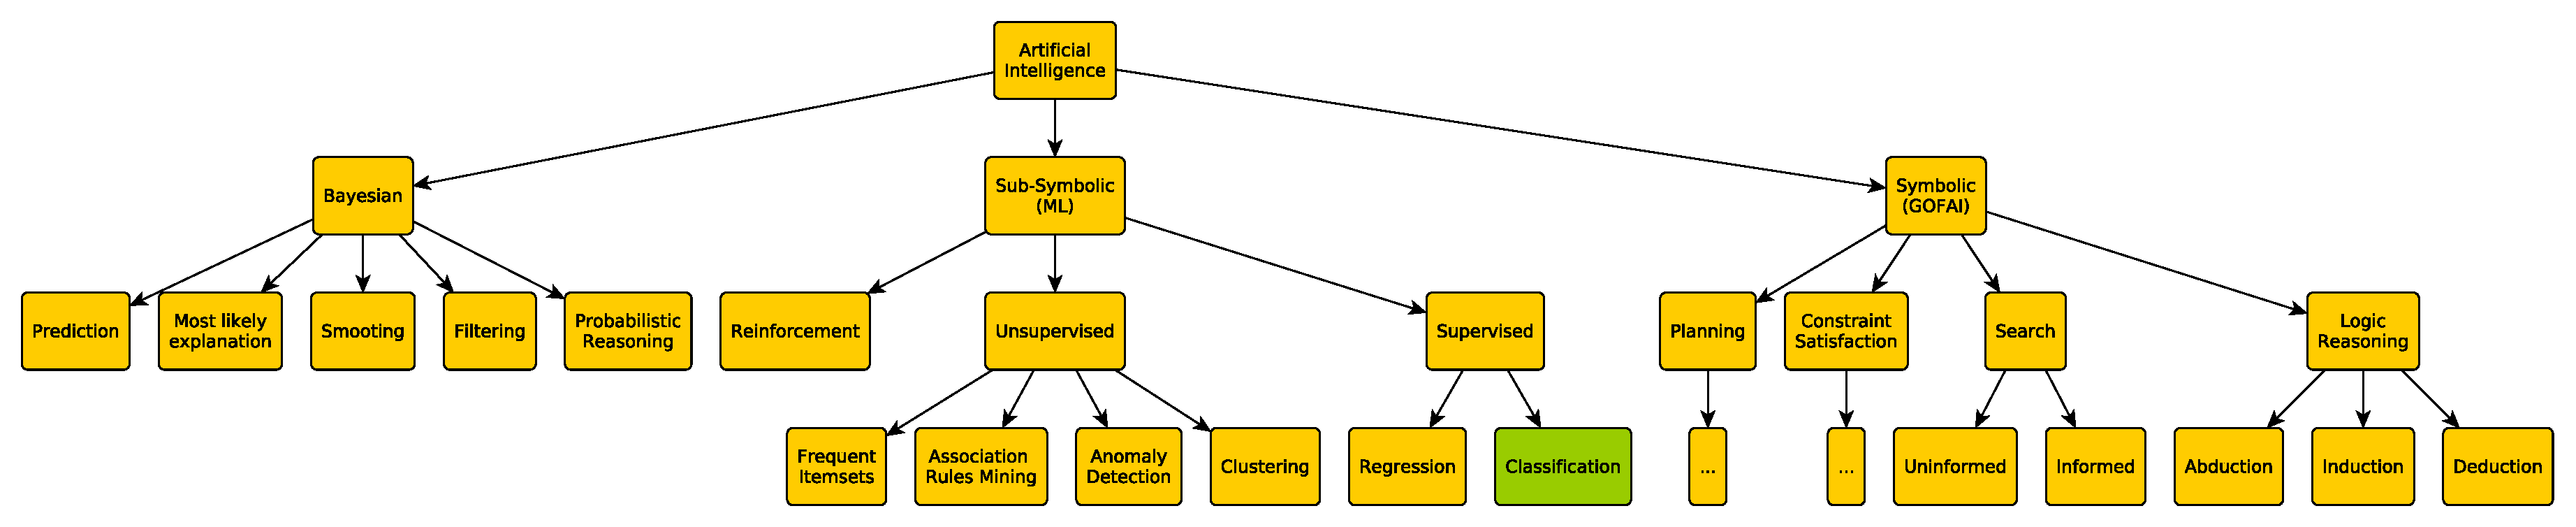
\includegraphics[width=.8\linewidth]{figures/random-image.pdf}
%     \caption{Some random image}
%     \label{fig:random-image}
% \end{figure}

% \section{Some cool topic}

% \part{Second Part}

% \chapter{Contribution}

% You may also put some code snippet (which is NOT float by default), eg: \cref{lst:random-code}.

% \lstinputlisting[float,language=Java,label={lst:random-code}]{listings/HelloWorld.java}

% \section{Fancy formulas here}

%----------------------------------------------------------------------------------------
% BIBLIOGRAPHY
%----------------------------------------------------------------------------------------

\backmatter

\part*{}

\nocite{*} % comment this to only show the referenced entries from the .bib file
\bibliographystyle{alpha}
\bibliography{phd-thesis}

\end{document}